\documentclass[11pt]{article}
\usepackage[spanish]{babel}
\usepackage{amsmath}
\usepackage{algorithm}
\usepackage{listings}
\usepackage{xcolor}
\usepackage{graphicx}
\usepackage{tabularx}
\usepackage{hyperref}

\newcommand\pythonstyle{\lstset{
language=Python,
basicstyle=\ttm,
morekeywords={self},              % Add keywords here
keywordstyle=\ttb\color{deepblue},
emph={},          % Custom highlighting
emphstyle=\ttb\color{deepred},    % Custom highlighting style
stringstyle=\color{deepgreen},
frame=tb,                         % Any extra options here
showstringspaces=false
}}



\title{Helk}
\author{Luis Ernesto Amat Cárdenas C-312 (MatCom)}
\date{\today}

\begin{document}

\maketitle

\section{Descripción General del Pipeline del Compilador}
El compilador sigue una arquitectura tradicional de múltiples etapas:

\begin{figure}[h]
\centering
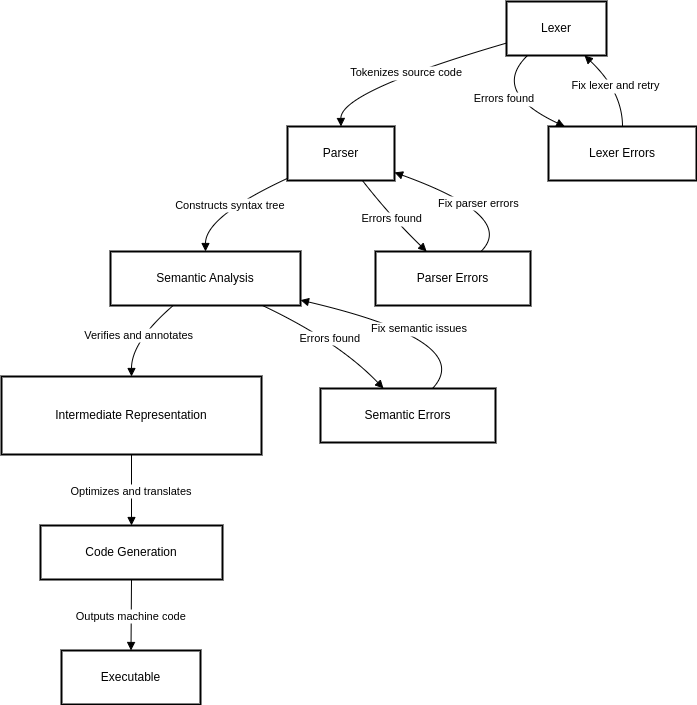
\includegraphics[width=0.8\textwidth]{compiler_pipeline.png}
\caption{Diagrama de arquitectura del compilador}
\end{figure}

Componentes principales:
\begin{itemize}
\item \textbf{Generador de Lexer}: Se genera código válido C que simula las transiciones del autómata finito determinista
\item \textbf{Generador de Parser}: Parser LL1 descendente recursivo con manejo de errores. Cuenta con un DSL propio para insertar código C.
\item \textbf{Análisis Semántico}: Enfoque basado en Problemas de Satisfacción de Restricciones (CSP) sobre la hipótesis de que a cada nodo le curresponde un único tipo
\item \textbf{Generación de Código}: Emisión directa de texto en formato LLVM IR con optimizaciones menores
\end{itemize}

\section{Introducción y Uso}
\subsection{Compilación del Proyecto}
\begin{lstlisting}[language=bash]
# Instalar dependencias
sudo apt install llvm clang

# Compilar proyecto
make compile

# Ejecutar pruebas
pytest test_compiler.py
\end{lstlisting}

\section{Análisis Léxico}
\subsection{Implementación del Generador de Lexer}
Implementación de la máquina de estados a partir de un conjunto de expresiones regulares:

\begin{enumerate}
    \item Expandir y simplificar la cada expresión regular ($[a-z] \leftarrow abcd...z$)
    \item Crear los autómatas finitos no deterministas (NFA) de cada expresión regular.
    \item Construir el autómata de la unión de todos los NFAs para definir el lenguaje que reconocerá el lexer.
    \item Convertir el NFA de la unión a un DFA (autómata finito determinista), respetando las prioridades de cada regla (keywords > itentifier)
    \item Simplificar rangos ($abcd...z \leftarrow 'a' =< x <= 'z'$)
    \item Generar el código para simular el autómata usando un alfabeto finito ($ASCII < 128$) usando swtich y goto
\end{enumerate}


Finalmente:

\begin{lstlisting}
Token* lexer(const char* input, int length, unsigned int* _num_tokens) {
    Token token;
    LexerState* lexer_init(state, input, length, true);

    while (state->current < state->end) {
        token = lexer_next_token(state);
    }
}
\end{lstlisting}

\section{Análisis Sintáctico}
\subsection{Implementación del Parser}

\begin{enumerate}
    \item Obtener la gramática a partir del DSL
    \item Generar la tabla (computar FIRST, FOLLOW, ...)
    \item Verificar que es realmente parseable por un parser LL1 usando la tabla (a.k.a. que no existan dos entradas en una misma casilla)
    \item Generar código C válido para un parser recursivo LL1 usando la tabla y recursividad (cada no terminal es una función)
    \item Manejo de errores usando el FOLLOW para recuperarse de errores y seguir parseando, con el afán de encontrar más errores
\end{enumerate}

\section{Análisis Semántico con CSP}
\subsection{Satisfacción de Restricciones}
Variables: $X = \{T_1, T_2, \ldots, T_n\}$ (tipos de nodos AST)

Dominios: $D = \{\text{double}, \text{string}, \text{tipo\_personalizado(s)}\}$

\subsection{Propagación de Restricciones}
\begin{lstlisting}
bool solve_constraints(ConstraintSystem* cs) {
    bool changed;
    bool res = true;
    do {
        changed = false;
        for(size_t i=0; i<cs->count; i++) {
            TypeConstraint* c = &cs->constraints[i];
            TypeInfo* t = c->expected;
            size_t expected = t->kind;
            size_t actual = c->node->type_info.kind;

            // Propagate concrete -> unknown
            if(expected != TYPE_UNKNOWN &&
               actual == TYPE_UNKNOWN) {

                c->node->type_info.kind = ((TypeInfo*) (c->expected))->kind;

                changed = true;
            }

            // Check for conflicts
            if(expected != TYPE_UNKNOWN &&
               actual != TYPE_UNKNOWN &&
               expected != actual) {
               fprintf(stderr, "ERROR - Literal type mismatch (current_type=%d); [%d, %d]\n", c->node->type, c->node->line, c->node->column);
               res = false;
            }
        }
    } while(changed);

    return res;
}
\end{lstlisting}

\section{Generación de Código}

\section{Optimizaciones}
\begin{table}[h]
\centering
\begin{tabularx}{\textwidth}{|l|X|}
\hline
\textbf{Optimización} & \textbf{Descripción} \\
\hline
Eliminación de Código Muerto & Elimina funciones no llamadas \\
Desvirtualización de Métodos & Reemplaza llamadas virtuales por directas \\
\hline
\end{tabularx}
\caption{Optimizaciones del compilador}
\end{table}

\section{Conclusión}
El compilador implementa un pipeline completo con enfoques novedosos:

\begin{itemize}
\item Generación de código directa para Lexer y Parser
\item DSLs con posibilidad de escribir código (a lá Lex y Yacc)
\item Inferencia de tipos basada en CSP
\item Emisión directa de IR
\end{itemize}

Trabajo futuro incluye optimizaciones de bucles e integración de recolección de basura.

\begin{thebibliography}{9}
\bibitem{dragon}
Aho, A. V., et al. \textit{Compilers: Principles, Techniques, and Tools}. 2ª ed., Addison-Wesley, 2006.

\bibitem{llvm}
Lattner, C. \textit{LLVM: An Infrastructure for Multi-Stage Optimization}. Tesis Doctoral, 2002.
\end{thebibliography}

\end{document}
